
\chapter{Formal Analysis and Verification} \label{chap:fav}
%----------------------------------------------------------------------
As the role of computers in human society is growing in ever faster pace, the consequences of any error are growing too. Consider, for example, the speed with which smarthones seized our pockets. They certainly brings many benefits, but as we become devpendent on the smartphones, any malfuncion or error in them can affect our life. From not having access to an important information to a direct danger, like in the case of motorists stranded by their mobile navigation in the middle of wilderness~\cite{appleMaps}.

Or consider the recent advances in the area of autonomous vehicles. Where an error in smartphones can only deprive us of an information, or provide an incorrect one, an error in a self-driving car can cause it to swerve into a wall with dire consequences for the passengers.

Common testing techniques, despite advances in this field, are still mostly reactive and can detect only known errors, for which a test was written, and can't provide a guarantee of correctness. That is, they can tell that "none of these specified errors happened," but can't tell whether the system is really free of errors with respect to a specification.

Formal methods, with roots in mathematical areas like theorem proving, on the other side frequently has the power to verify the correctness. But unlike the common testing techniques, and despite an interest of the industry, they are not yet widely used. A notable exception to this is a {\em static analysis}, which, in some of its weaker forms, is becoming a part of integrated development environments (IDE) like Xcode or Eclipse~\cite{xcodeAnalysis}.

A part of the reason for the small adoption of formal methods is their complexity. They either require advanced user knowledge, like a human-driven deductions in {\em theorem proving}, require excessive modelling of the environment for the system like {\em model checking}, or are simply unable to cope with the size of the code and the size of it's state space.

By the term {\em formal analysis}, we describe methods for answering questions other than whether the tested system is free of errors with respect to some specification. That is, it includes questions like whether the program is guaranteed to always terminate, if a buffer size is bound and so on.

{\em Formal verification} then denotes methods capable of proving errorlessness of the given system with respect to correctness specification. {\em Completness} of a method is a property guaranteeing that it won't raise a false alarm, while if a method that is {\em sound} terminates and tells that there are no erros, the system is indeed correct.

In the following parts of this work, we will first discuss some of the formal techniques (the rest of this chapter) and then also their usefullness on a real, production code in the chapter~\nameref{chap:techniques}. We will look not only on their result, but also on the cost of using them, both in timew and expertise necessary for their correct use.

%======================================================================
\section{Static Analysis}\label{chap:fav:staticAnalysis}
%----------------------------------------------------------------------
A rather broad, but commonly used definition of {\em static analysis} is that it is an analysis that collects some information about the behaviour of a system without actually executing it under its original semantics~\cite[Chap. 2.2]{KrenaVojnarOverview}. It can manage a really big systems in a reasonable time and is highly automated, but can suffer false positivesand is generally weaker than other methods (it is difficult to express some problems for {\em static analysis}). This category includes methods:

{\em Abstract interpretation}, in which an abstract overrepresentation of the statements of the program is evaluated in an abstract machine for all possible inputs at once and we exchange completness for speed or even the possibility to analyse the system.

{\em Data flow analysis} tracks how a given set of properties propagates through the program without directly exectuting it.

{\em Error patterns} then denote the probably most common method used in various lightweight implementations already present in various IDEs, in Lint and Cppcheck software, and others. As the name itself explains, this methods attempts to detect commonly occuring patterns that programmers make, but which lead to an error. A simple example may be a missing {\tt break} statement, or missing boundary checks before accessing an array.

Let us now look more in the detail on each of these methods and on their implementations, but bear in mind that in many cases, the tools we will see are not clearly distinguished and can be placed into more than one category. Thus, the tools are categorised according to the most important principles in their implementation.

% ......
\subsection{Error patterns}
Tools using it: Lint~\cite{KrenaVojnarOverview} (and it's followers), cppcheck\footnote{I'm not sure about this and didn't found it cited anywhere, but from its code it looks like they search for error patterns.}

{\em Error patterns} detection is a rather wide array of different techniques and methods with a common goal: To detect more or less frequent type of errors. The great advantage of this class of methods is that they usually don't require any deeper knowledge, are fully automated and can very fast. Their disadvantages are that they are limited to a very specific kind of errors\footnote{Basically, every error pattern needs is own filter and only some kinds of error patterns are generic enough to be shipped within the tool. Consider a support for usage of a library. It makes sense to watch for patterns in usage of {\tt stdlib.h}, but how it should know patterns in a custom library? And even if the specific library is publicly available, including everything is impossible. Many tools allows for providing of custom definitions of these patterns, but from a personal experience, they are rarely used.} and suffers false positives.

An example of the approches used in this class of static analysis is detection of matching pairs of functions. For example, any {\tt open()} call should be later followed with one {\tt close()} in every possible path. Or a state machine can be used to detect missing delimiter between statements or a missing {\tt break} in a {\tt switch}~\cite{dynamine}.

\subsubsection{Lint}
Lint was originally created in the 70's for early C language~\cite[Chap. 2.2]{KrenaVojnarOverview} and since then, multiple new tools for various languages was inspired by it: splint, cpplint, JSLint, Pylint, etc. It searches for patterns that are likely to be bugs, to be non-portable, or to be wasteful~\cite{lintMan}. Many of the follower implementations are open-source.

\subsubsection{CppCheck}
An open-source tool for C/C++ languages. It can only a very simple {\em control flow analysis}, where it expects that all statements can be always either true or false and thus all statements should be always reachable~\cite{cppcheckDesign}.

% ......
\subsection{Data flow analysis}
Tools using it: Coverity~\cite{KrenaVojnarOverview}, CodeSonar~\cite{KrenaVojnarOverview}, TruePath~\cite{KrenaVojnarOverview}, FindBugs~\cite{KrenaVojnarOverview}

These methods, in industrial tools frequently combined with {\em error patterns}, tracks how so-called {yem data flow facts} propagate between within a {\em control flow graph} between its nodes. These nodes represents {\em basic blocks} in the original code, each block having only one entry point and one exit point\footnote{One entry point means that in no case can any instruction inside of the block other than the first one be a target of a jump. One exit point means that if there is a branching, only the last instruction of a block can cause it and jump to multiple different target instructions.}, which simplifies the analysis.

The analysis can be either {\em forward}, where the state at the exit of one basic block is used as the input of the following block and which starts at the beginning of the program. Or {\em backwards analysis}, where the algorithm starts in an end state and attempts to find a path to a start state. This second approach can be useful to determine whether a particular end configuration is reachable.

\subsubsection{Coverity}
A proprietary tool (and company) providing a free service for open-source projects (\url{http://scan.coverity.com}). Uses restricted formal verification, but getting to specific details is hard or impossible. Supports languages Java, C/C++, C\#, JavaScript, Ruby, and Python.

\subsubsection{FindBugs}
FindBugs is an open-source code analyser for Java langauge with plugins for many Java IDEs.

% ......
\subsection{Abstract interpretation}
Tools using it: Astrée~\cite{Astree1,KrenaVojnarOverview}, PolySpace~\cite{KrenaVojnarOverview}

{\em Abstract interpretation} shares a blurry border with {\em model checking} and it may be different to determine where a specific method is. The basic way of how abstract interpretation works is to run a symbolic execution of the program. On every statement, transform specific values into an abstract context and {\em widen} (over-approximate) or {\em narrow} to refine the result after widening.

The widening and narrowing is usually implemented by using a pair of monotone functions: {\em Abstraction} denoted $\alpha$ and {\em concretisation} denoted $\gamma$ forms a Galois connection.

These methods can be sound, but not every abstract interpretation is, as they can range from a simple syntax analyser to full model checking.

\subsubsection{Astrée}
A tool for analysing applications written in C language. It is a proprietary tool used for safety-critical applications, for example by Airbus~\cite{KrenaVojnarOverview}. It provides a sound static analysis. False positives are considered a reasonable price for the soundess~\cite{Astree1}.

\subsubsection{PolySpace}
A proprietary tool for C, C++, and Ada languages.

%======================================================================
\section{Model Checking}\label{chap:fav:modelChecking}
%----------------------------------------------------------------------
Tools using it: RuleBase~\cite{KrenaVojnarOverview}, Incisive VErifier~\cite{KrenaVojnarOverview}, Magellan~\cite{KrenaVojnarOverview}, JasperGold Formal Property Verification App~\cite{KrenaVojnarOverview}, Questa Formal Verification~\cite{KrenaVojnarOverview},CPAchecker~\cite{KrenaVojnarOverview}, Wolverine~\cite{KrenaVojnarOverview}, CBMC~\cite{KrenaVojnarOverview}, LLBMC~\cite{KrenaVojnarOverview}

{\em Model checking} is an algoritmic mean of checking whether the given system is correct with regards to any given property through systematic exploring of state space of this system. The properties are usually specified in some temporal logic like LTL, CTL, CTL* or $\mu$-calculus.

The advantages of {\em model checking} are that it can be fully automated, is rather universal, doesn't require a deep knowledge for usage and if it finds an error, it can generate a path leading to the case, which is usefull for repairs.

However, it also has two big disadvantages. It requires a model of the environment for the system and suffers {\em state space explosion}. The number of reachable space grows exponentially -- consider a 32bit variable, which has $2^{32}$ possible values, which equals states. That means that $n$ of such variables equals $2^{32\times n}$ states. The result is that any attempt in a practical use of {\em model checking} has to cope with this state space explosion.

\begin{wrapfigure}{r}{8cm}
  \centering
 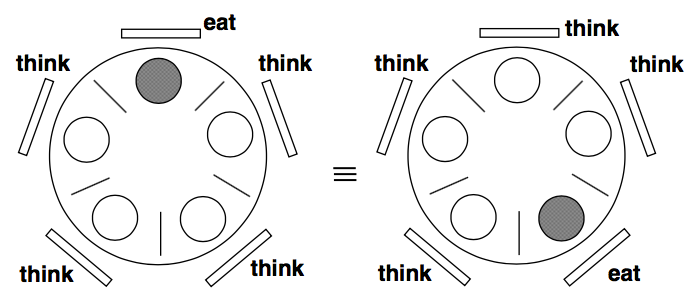
\includegraphics[width=8cm,keepaspectratio]{fig/dinning-symmetry} % Or .pdf
\caption{Symmetries and the dinning philosophers~\cite{KrenaVojnarOverview}.}
\label{fig:fav:dinning}
\end{wrapfigure}

The methods used for this include {\em symmetry reduction} in cases where it is not important which specific entity (if there is more entities of the same type is in a specific state). See figure~\ref{fig:fav:dinning} for an example of symmetry in the well known dinning philosophers problem.

Other solutions can be to use only one of many possible pathes for ordering of concurent actions that are independent of each other and compress the size of states by using pointers to the previous state for values that didn't changed. Or the tool can evaluate the properties at the same time when a new state is generated, and stop immediately once it is clear that this prefix cannot be accepted by the automata denoting correctness specification.


\subsubsection{CPAChecker}
An open-source tool and a framework for analysis of programs in C language. It is based on the idea of {\em configurable program analysis}~\cite{CPAChecker}, which uses user configuration to perform a reachability analysis.


%======================================================================
\section{Theorem Proving}\label{chap:fav:theoremProving}
%----------------------------------------------------------------------
Tools using it: VCC~\cite{KrenaVojnarOverview}, ESC/Java2~\cite{KrenaVojnarOverview}, VS3~\cite{KrenaVojnarOverview}

{\em Theorem proving} is similar to mathematical deduction, where we get a proof from an initial set of axioms. It also shares advantages and disadvantages with its purely mathematical counterpart. On the one side, it is really universal, but on the other side, it can't provide a {\em counterexample} (a path to an error), but just says yes/no, and is only semiautomatic. The tools can correctly apply inference rules, but their choice is on the user. Thus, an insufficiently skilled user may not be able to prove that the system is correct even if there are no errors in the system.


